% Modelo do artigo. Os marcadores entre sinais de porcentagem duplos são preenchidos por gerar_tabelas.py,
% que grava artigo.tex com os números de resultados/. Edite este arquivo, não o artigo.tex.
\documentclass[12pt]{article}

\usepackage{sbc-template}
\usepackage{graphicx,url}
\usepackage[utf8]{inputenc}
\usepackage[T1]{fontenc}
\usepackage[brazil]{babel}
\usepackage{amsmath,amssymb}
\usepackage{booktabs}

\graphicspath{{../figuras/}}

\sloppy

\title{Otimização de Dietas para Atletas e Pessoas\\com Restrições Alimentares}

\author{Antonio Soares Couto Neto\inst{1}, Rodrigo Drummond\inst{1}, Thales Matheus\inst{1}}

\address{Pontifícia Universidade Católica de Minas Gerais (PUC Minas)\\
Belo Horizonte -- MG -- Brasil}

\begin{document}

\maketitle

\begin{abstract}
This paper models the diet problem for nine nutritional profiles (reference adult,
overweight, underweight, strength athlete, vegetarian, vegan, lactose intolerant,
celiac and vegetarian athlete) over 37 Brazilian foods and nine nutrients, with seven
objective functions plus weighted-sum and $\varepsilon$-constraint formulations. Three
solvers were implemented from scratch: a two-phase Simplex with shadow-price
extraction, a Branch and Bound for integer servings and a memetic Genetic Algorithm
with Deb's feasibility rules. The Simplex and the Branch and Bound matched the CBC
solver in all 90 cases, solving each linear model in %%TEMPO_LP%% ms and each integer
model in %%BB_TEMPO%% s on average. The dual analysis shows what makes each diet
expensive: one extra gram of protein costs R\$ %%DUAL_PROT_ATL%% for the athlete and
%%DUAL_PROT_PCT%%\% more without meat, and iron costs R\$ %%DUAL_FE_VEG%% per mg for
vegetarians. Integer servings raise the cost by %%GAP_INT%%\% over the linear
relaxation, and the Genetic Algorithm stayed %%GA_GAP%%\% above the optimum on average.
\end{abstract}

\begin{resumo}
Este artigo modela o problema da dieta para nove perfis nutricionais (adulto de
referência, sobrepeso, subpeso, atleta de força, vegetariano, vegano, intolerante à
lactose, celíaco e atleta vegetariano) com 37 alimentos brasileiros e nove nutrientes,
sete funções objetivo e as formulações de soma ponderada e $\varepsilon$-restrito. Três
métodos foram implementados do zero: Simplex de duas fases com cálculo dos
preços-sombra, Branch and Bound para porções inteiras e um Algoritmo Genético memético
com as regras de factibilidade de Deb. Simplex e Branch and Bound coincidiram com o
resolvedor CBC nos 90 casos, resolvendo cada modelo linear em %%TEMPO_LP%%~ms e cada
modelo inteiro em %%BB_TEMPO%%~s, em média. A análise dual mostra o que encarece cada
dieta: um grama a mais de proteína custa R\$~%%DUAL_PROT_ATL%% ao atleta e
%%DUAL_PROT_PCT%%\% a mais sem carnes, e o ferro custa R\$~%%DUAL_FE_VEG%% por mg ao
vegetariano. Porções inteiras encarecem a dieta em %%GAP_INT%%\% sobre a relaxação
linear, e o Genético ficou em média %%GA_GAP%%\% acima do ótimo.
\end{resumo}

\section{Introdução}

O problema da dieta é um dos problemas clássicos da Programação Linear. \cite{stigler1945}
buscou a combinação mais barata de alimentos capaz de atender às necessidades nutricionais
de um adulto, e o problema foi um dos primeiros resolvidos pelo método Simplex
\cite{dantzig1963,dantzig1990}. Desde então, a Programação Linear vem sendo usada para
formular dietas de baixo custo, recomendações alimentares para populações e dietas com
menor impacto ambiental \cite{vandooren2018}.

A necessidade nutricional, porém, varia de pessoa para pessoa. Atletas precisam de mais
energia e proteína \cite{thomas2016}; quem busca emagrecer precisa de déficit calórico sem
perder massa magra; vegetarianos precisam de mais ferro, porque o ferro de origem vegetal
é menos absorvido \cite{iom2006,melina2016}; intolerantes à lactose e celíacos precisam
excluir alimentos inteiros. Essas condições também se somam, como no atleta vegetariano.
Cada perfil muda as restrições do modelo e, com elas, a dieta ótima e o que a encarece.

A formulação clássica tem ainda duas limitações práticas. A primeira é que a solução
linear tem porções fracionárias (0,37 copo de leite, por exemplo), que precisam ser
arredondadas sem perder a factibilidade. A segunda é que custo mínimo não é o único
critério relevante: um atleta pode querer mais proteína, e um hipertenso, menos sódio.
Isso pede funções objetivo alternativas, uma análise de compromisso entre critérios e
métodos de solução além do Simplex.

Este trabalho trata essas questões com o Nutriliza, um modelo de otimização de dietas
com nove perfis, 37 alimentos brasileiros e nove nutrientes. O modelo é resolvido por
três métodos implementados pelo grupo: o Simplex de duas fases, com cálculo dos
preços-sombra; o Branch and Bound, para porções inteiras; e um Algoritmo Genético
memético. A contribuição do trabalho é tripla: formular o problema da dieta para perfis
com restrições simultâneas, usar a análise dual e as fronteiras de Pareto para mostrar
o que encarece cada dieta, e comparar um método exato e uma metaheurística no modelo
de porções inteiras. O código, os dados e os resultados estão em
\url{https://github.com/nietus/Nutriliza}.

O restante do artigo está organizado como segue. A Seção~\ref{sec:trabalhos} posiciona o
trabalho na literatura; a Seção~\ref{sec:metodologia} formaliza o problema e detalha os
métodos; a Seção~\ref{sec:resultados} apresenta os experimentos; e a
Seção~\ref{sec:conclusao} resume os achados e as limitações.

\section{Trabalhos Relacionados}\label{sec:trabalhos}

\cite{stigler1945} estimou o custo mínimo de uma dieta para um homem adulto com 77
alimentos e nove nutrientes, chegando a uma solução heurística. O problema foi depois
resolvido de forma exata pelo Simplex, em um dos primeiros grandes cálculos de
Programação Linear \cite{dantzig1990}. A revisão de \cite{vandooren2018} mostra que a
formulação continua em uso, agora com objetivos nutricionais, econômicos e ambientais.
\cite{darmon2002} usaram programação linear e não linear para identificar
nutrientes-problema em dietas infantis, ideia próxima da análise de preços-sombra feita
aqui: em vez de olhar só a dieta ótima, olha-se quais exigências limitam a solução.

Para variáveis inteiras, o Branch and Bound de \cite{landdoig1960} é a base dos
resolvedores atuais, como o CBC \cite{forrest2005}. Algoritmos Genéticos
\cite{holland1975,goldberg1989} são uma alternativa quando o modelo deixa de ser linear,
e o tratamento de restrições de \cite{deb2000}, sem pesos de penalidade, evita a etapa de
calibração. Problemas com mais de um critério podem ser tratados pela soma ponderada ou
pelo método $\varepsilon$-restrito \cite{haimes1971,miettinen1999}; este último encontra
também os pontos da fronteira que a soma ponderada não alcança.

\section{Metodologia}\label{sec:metodologia}

\subsection{Formulação do Problema}

Seja $x_i$ o número de porções diárias do alimento $i$, $a_{ji}$ a quantidade do
nutriente $j$ em uma porção do alimento $i$, $L_j$ e $U_j$ os limites do perfil, $g_i$ o
peso da porção, $M_i$ o máximo de porções e $FH$ o conjunto de frutas e hortaliças. O
modelo é:
\begin{align}
\min \text{ ou } \max \quad & Z = \textstyle\sum_{i=1}^{n} c_i x_i \label{eq:fo}\\
\text{s.a.} \quad & L_j \leq \textstyle\sum_{i=1}^{n} a_{ji} x_i \leq U_j, & j = 1,\dots,m \label{eq:nut}\\
& \textstyle\sum_{i \in FH} g_i x_i \geq 400 \label{eq:fh}\\
& 0 \leq x_i \leq M_i, \quad x_i = 0 \text{ se } i \text{ é proibido pelo perfil}, & i = 1,\dots,n \label{eq:lim}
\end{align}
A restrição~(\ref{eq:fh}) segue a recomendação da OMS de 400~g diários de frutas e
hortaliças \cite{who2003}, e $M_i$ evita dietas monótonas. No modelo linear as porções
são contínuas; no modelo inteiro, $x_i \in \mathbb{Z}$, o que gera porções que podem ser
servidas.

Para o custo mínimo, escrevendo as restrições de máximo como
$-\sum_i a_{ji} x_i \geq -U_j$, o primal fica na forma $\min c^\top x$ s.a.
$Ax \geq b$, $x \geq 0$, e o dual é $\max b^\top y$ s.a. $A^\top y \leq c$, $y \geq 0$.
No ótimo, $y_j$ é o preço-sombra da restrição $j$: quanto o custo mínimo sobe se $b_j$
aumentar uma unidade. Pela folga complementar, só restrições ativas têm $y_j \neq 0$.

Sete funções objetivo foram implementadas: minimizar custo, calorias, sódio, gordura ou
peso total, e maximizar proteína ou fibra. Para dois critérios ao mesmo tempo, usam-se a
soma ponderada $Z = w\,\text{custo}/\text{custo}^* + (1-w)\,\text{sódio}/\text{sódio}^*$,
com os ótimos individuais como normalização, e o método $\varepsilon$-restrito, que
minimiza o custo com o outro critério como restrição e varia $\varepsilon$.

\subsection{Instâncias e Cenários}

A base tem 37 alimentos comuns no Brasil (cereais, tubérculos, leguminosas, carnes,
ovos, laticínios, oleaginosas, frutas e hortaliças), com composição por 100~g retirada
da Tabela Brasileira de Composição de Alimentos \cite{taco2011} e, para tofu, bebida de
soja e whey, de rótulos. Cada alimento tem uma porção caseira (1 concha de feijão =
140~g, por exemplo), um preço (premissa de mercado de Belo Horizonte em 2026) e
marcadores de carne, origem animal, lactose e glúten. Os nove nutrientes são energia,
proteína, carboidrato, gordura, fibra, cálcio, ferro, sódio e vitamina~C.

A Tabela~\ref{tab:perfis} resume os nove perfis. Os limites seguem as DRIs
\cite{iom2006}, o limite de sódio da OMS \cite{who2012} e o consenso de nutrição
esportiva \cite{thomas2016}; para vegetarianos, o ferro mínimo é 1,8 vez maior. Todos
os perfis exigem também 1.000 a 2.500~mg de cálcio, ao menos 75~mg de vitamina~C
(90~mg para atletas) e no máximo 2.000~mg de sódio (2.300~mg no subpeso e 3.000~mg para
atletas). Cada perfil combinado com cada função objetivo forma uma instância, o que dá
63 instâncias lineares; o modelo inteiro foi resolvido para os 9 perfis com três
funções objetivo (custo, sódio e peso total), em 27 instâncias.

\begin{table}[ht]
\centering
\caption{Perfis nutricionais e limites diários.}\label{tab:perfis}
\footnotesize
\begin{tabular}{lcccccl}
\toprule
Perfil & Energia (kcal) & Prot. (g) & Carb. (g) & Gord. (g) & Ferro (mg) & Exclui \\
\midrule
Referência & 2.000--2.400 & 60--140 & 250--360 & 45--85 & 8--45 & -- \\
Sobrepeso & 1.500--1.700 & 90--130 & 130--200 & 35--55 & 8--45 & -- \\
Subpeso & 2.800--3.200 & 80--140 & 380--480 & 75--110 & 8--45 & -- \\
Atleta & 3.000--3.400 & 130--180 & 400--520 & 60--110 & 8--45 & -- \\
Vegetariano & 2.000--2.400 & 60--140 & 250--360 & 45--85 & 14--45 & carnes \\
Vegano & 2.000--2.400 & 60--140 & 250--360 & 45--85 & 14--45 & prod. animais \\
Intol. à lactose & 2.000--2.400 & 60--140 & 250--360 & 45--85 & 8--45 & lactose \\
Celíaco & 2.000--2.400 & 60--140 & 250--360 & 45--85 & 8--45 & glúten \\
Atleta vegetariano & 3.000--3.400 & 130--180 & 400--520 & 60--110 & 14--45 & carnes \\
\bottomrule
\end{tabular}

\end{table}

\subsection{Algoritmos Comparados}

Os três métodos foram implementados em Python com NumPy. O CBC \cite{forrest2005},
chamado pela biblioteca PuLP \cite{mitchell2011}, serviu apenas para validar os
resultados.

\textbf{Simplex de duas fases.} As variáveis são deslocadas pelo limite inferior, os
limites superiores viram restrições e entram folgas, excessos e artificiais. A fase~1
minimiza a soma das artificiais; mínimo positivo indica perfil inviável. A fase~2
otimiza $Z$ escolhendo a coluna de custo reduzido mais negativo (regra de Dantzig) e
passa à regra de \cite{bland1977} após 50 pivôs degenerados seguidos, o que impede
ciclos. Os preços-sombra saem de $y^\top = c_B^\top B^{-1}$, resolvendo
$B^\top y = c_B$ na base ótima.

\textbf{Branch and Bound.} Cada nó é o modelo com limites de variável mais apertados, e
sua relaxação linear é resolvida pelo Simplex próprio. A variável mais fracionária
$x_j$ gera os ramos $x_j \leq \lfloor x_j \rfloor$ e $x_j \geq \lceil x_j \rceil$. A
busca mergulha em profundidade até a primeira solução inteira e depois explora o nó de
melhor limite. Há poda por inviabilidade, por limite e por integralidade, e uma
heurística de arredondamento em cada nó gera soluções inteiras cedo.

\subsection{Algoritmo Genético Memético}

O cromossomo é o vetor de porções inteiras em $[0, M_i]$. As restrições são tratadas
pelas regras de \cite{deb2000} no torneio binário: factível vence infactível, entre
factíveis vence o melhor objetivo e entre infactíveis vence a menor violação
normalizada. Os operadores são cruzamento uniforme (taxa 0,9), mutação de $\pm 1$
porção (taxa $1{,}5/n$) com reinício ocasional do gene e elitismo dos seis melhores.
Os indivíduos de elite passam por descida na vizinhança de $\pm 1$ porção e de troca de
uma porção entre dois alimentos, o que torna o algoritmo memético. Usaram-se população
de 200, 500 gerações e 10 sementes por instância.

\section{Resultados}\label{sec:resultados}

Os experimentos rodaram em um notebook com Windows 11 e Python 3.14. O Simplex
resolveu as 63 instâncias lineares com os mesmos valores ótimos e preços-sombra do CBC
(diferença abaixo de $10^{-6}$), em média com %%PIVOS%% pivôs.

\subsection{Custo Mínimo por Perfil}

A Tabela~\ref{tab:custo} mostra a dieta de custo mínimo de cada perfil. A do adulto de
referência custa R\$~%%CUSTO_REF%% por dia e já não contém glúten, por isso o perfil
celíaco custa o mesmo: excluir um alimento só encarece a dieta se ele estiver na
solução ótima. O atleta custa R\$~%%CUSTO_ATL%% (%%ATL_PCT%%\% a mais), e somar a
exclusão de carnes eleva o custo para R\$~%%CUSTO_ATLV%%. As exclusões também aumentam
o número de pivôs, porque a base inicial fica mais distante do ótimo.

\begin{table}[ht]
\centering
\caption{Dieta de custo mínimo por perfil (modelo linear).}\label{tab:custo}
\footnotesize
\begin{tabular}{lrrrrrrr}
\toprule
Perfil & Custo (R\$) & kcal & Prot. (g) & Fibra (g) & Ferro (mg) & Sódio (mg) & Pivôs \\
\midrule
Referência & 9{,}00 & 2.000 & 62 & 58 & 8{,}0 & 434 & 52 \\
Sobrepeso & 10{,}37 & 1.500 & 90 & 45 & 9{,}1 & 584 & 40 \\
Subpeso & 11{,}62 & 2.800 & 83 & 55 & 8{,}1 & 409 & 58 \\
Atleta & 14{,}11 & 3.000 & 130 & 79 & 18{,}2 & 617 & 53 \\
Vegetariano & 9{,}77 & 2.000 & 73 & 70 & 14{,}0 & 305 & 87 \\
Vegano & 10{,}62 & 2.000 & 70 & 72 & 14{,}0 & 48 & 116 \\
Intol. à lactose & 9{,}30 & 2.000 & 62 & 45 & 9{,}7 & 824 & 56 \\
Celíaco & 9{,}00 & 2.000 & 62 & 58 & 8{,}0 & 434 & 56 \\
Atleta vegetariano & 14{,}21 & 3.000 & 130 & 85 & 19{,}5 & 603 & 61 \\
\bottomrule
\end{tabular}

\end{table}

\subsection{Comparação entre Funções Objetivo}

A Tabela~\ref{tab:conflito} avalia, para o atleta, a dieta ótima de cada função
objetivo em todos os critérios. Maximizar proteína leva ao teto de 180~g, mas custa
R\$~%%CUSTO_PROT%% contra R\$~%%CUSTO_ATL%% da dieta mais barata; minimizar o peso
total gera a dieta mais concentrada, mas com %%SODIO_MASSA%%~mg de sódio. Minimizar
calorias ou gordura apenas encosta nos limites mínimos do perfil: nesses casos, os
limites pesam mais que o critério.

\begin{table}[ht]
\centering
\caption{Atleta: dieta ótima de cada função objetivo avaliada em todos os critérios.}\label{tab:conflito}
\footnotesize
\begin{tabular}{lrrrrrr}
\toprule
Função objetivo & Custo (R\$) & kcal & Prot. (g) & Fibra (g) & Sódio (mg) & Peso (g) \\
\midrule
Minimizar custo & 14{,}11 & 3.000 & 130 & 79 & 617 & 2.795 \\
Minimizar calorias & 14{,}11 & 3.000 & 130 & 79 & 617 & 2.795 \\
Maximizar proteína & 18{,}28 & 3.000 & 180 & 73 & 704 & 2.765 \\
Maximizar fibra & 32{,}87 & 3.400 & 152 & 135 & 870 & 2.985 \\
Minimizar sódio & 21{,}10 & 3.225 & 130 & 97 & 55 & 2.466 \\
Minimizar gordura & 14{,}11 & 3.000 & 130 & 79 & 617 & 2.795 \\
Minimizar quantidade total & 25{,}78 & 3.000 & 130 & 44 & 1.891 & 1.230 \\
\bottomrule
\end{tabular}

\end{table}

\subsection{Análise Dual}

A Tabela~\ref{tab:duais} traz os preços-sombra das restrições ativas na dieta de custo
mínimo, em reais por unidade. Cada grama a mais de proteína custa R\$~%%DUAL_PROT_ATL%%
ao atleta e R\$~%%DUAL_PROT_ATLV%% ao atleta vegetariano (%%DUAL_PROT_PCT%%\% a mais).
O ferro custa R\$~%%DUAL_FE_REF%% por mg ao adulto de referência e
R\$~%%DUAL_FE_VEG%% ao vegetariano: é a exigência que mais pesa para quem não come
carne. No perfil de sobrepeso, o preço-sombra do teto de carboidrato é negativo, ou
seja, afrouxá-lo baratearia a dieta, porque os alimentos mais baratos são ricos em
carboidrato. A energia tem preço-sombra baixo em todos os perfis: calorias são
baratas, e o que encarece a dieta são proteína, ferro, cálcio e gordura.

\begin{table}[ht]
\centering
\caption{Preços-sombra na dieta de custo mínimo (R\$ por unidade; ``--'' indica
restrição não ativa).}\label{tab:duais}
\footnotesize
\begin{tabular}{lrrrrrrr}
\toprule
Restrição & Ref. & Sobrep. & Subp. & Atleta & Veget. & Vegano & Atl. veg. \\
\midrule
Energia mín. (kcal) & 0{,}0019 & 0{,}0018 & 0{,}0029 & 0{,}0004 & 0{,}0015 & 0{,}0019 & $<$0{,}0001 \\
Proteína mín. (g) & -- & 0{,}0783 & -- & 0{,}0834 & -- & -- & 0{,}1057 \\
Carboidrato máx. (g) & -- & -0{,}0114 & -- & -- & -- & -- & -- \\
Gordura mín. (g) & 0{,}0231 & -- & 0{,}0341 & 0{,}0218 & 0{,}0267 & 0{,}0234 & 0{,}0156 \\
Cálcio mín. (mg) & 0{,}0029 & 0{,}0021 & 0{,}0024 & 0{,}0017 & 0{,}0030 & 0{,}0049 & 0{,}0016 \\
Ferro mín. (mg) & 0{,}0838 & -- & -- & -- & 0{,}2355 & 0{,}0661 & -- \\
Frutas e hortaliças (g) & 0{,}0032 & 0{,}0038 & 0{,}0030 & 0{,}0033 & 0{,}0025 & 0{,}0021 & 0{,}0032 \\
\bottomrule
\end{tabular}

\end{table}

\subsection{Fronteiras de Pareto}

A Figura~\ref{fig:pareto}(a) aplica o método $\varepsilon$-restrito a custo e proteína.
As curvas são lineares por partes, e a inclinação de cada trecho é o preço-sombra da
proteína naquele intervalo, o que liga a análise dual à análise multiobjetivo. A curva
do vegano cresce mais rápido: sem produtos animais, cada grama de proteína a mais fica
cada vez mais caro. Na Figura~\ref{fig:pareto}(b), a soma ponderada só encontra
vértices da fronteira custo $\times$ sódio, enquanto o $\varepsilon$-restrito traça a
curva inteira.

\begin{figure}[ht]
\centering
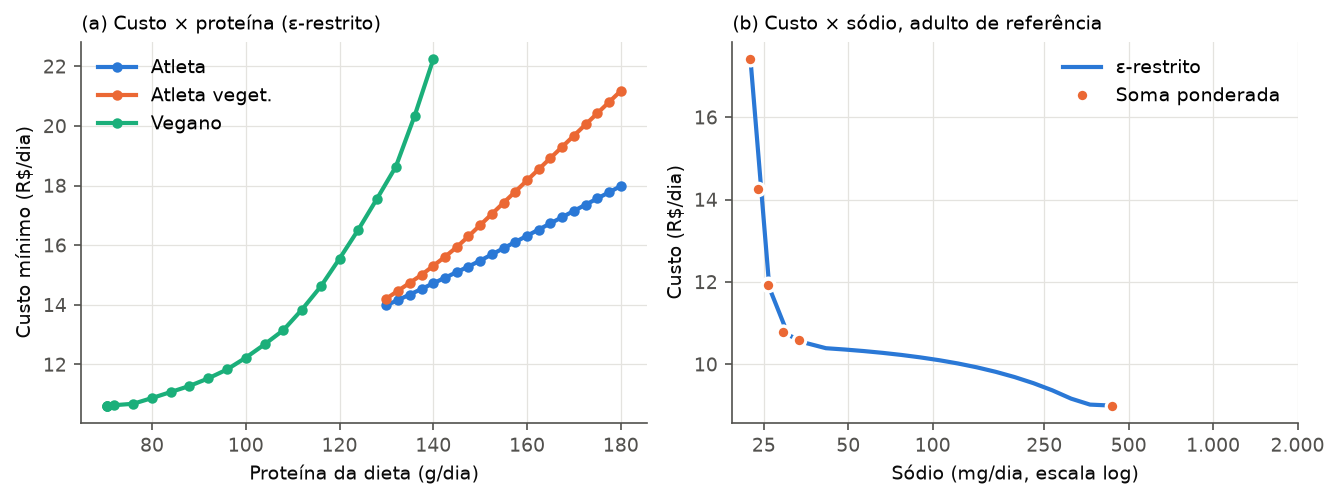
\includegraphics[width=\textwidth]{pareto.png}
\caption{Fronteiras de Pareto: (a) custo $\times$ proteína; (b) custo $\times$ sódio.}\label{fig:pareto}
\end{figure}

\subsection{Branch and Bound versus Algoritmo Genético}

O Branch and Bound chegou ao ótimo nas 27 instâncias inteiras, igual ao CBC, com média
de %%BB_NOS%% nós (máximo de %%BB_NOS_MAX%%). Exigir porções inteiras encarece a dieta
em média %%GAP_INT%%\% em relação à relaxação linear. O Genético achou soluções
factíveis em todas as %%GA_EXEC%% execuções, mas ficou em média %%GA_GAP%%\% acima do
ótimo e chegou ao ótimo em %%GA_OTIMO%%\% delas. O desvio médio foi de
%%GA_GAP_CUSTO%%\% no custo, %%GA_GAP_SODIO%%\% no sódio e %%GA_GAP_MASSA%%\% no peso
total, com pior caso de %%GA_GAP_MAX%%\% (Tabela~\ref{tab:inteiro}).

\begin{table}[ht]
\centering
\caption{Custo mínimo com porções inteiras (R\$): relaxação linear, Branch and Bound e
Algoritmo Genético (10 sementes).}\label{tab:inteiro}
\footnotesize
\begin{tabular}{lrrrrrr}
\toprule
Perfil & LP & B\&B & Nós & B\&B (s) & AG média $\pm$ dp & AG no ótimo \\
\midrule
Referência & 9{,}00 & 9{,}48 & 940 & 1{,}7 & 9{,}84 $\pm$ 0{,}12 & 0\% \\
Sobrepeso & 10{,}17 & 10{,}70 & 856 & 1{,}5 & 11{,}27 $\pm$ 0{,}30 & 0\% \\
Subpeso & 11{,}62 & 12{,}03 & 250 & 0{,}4 & 12{,}40 $\pm$ 0{,}22 & 10\% \\
Atleta & 13{,}99 & 14{,}45 & 462 & 1{,}0 & 14{,}97 $\pm$ 0{,}21 & 10\% \\
Vegetariano & 9{,}77 & 10{,}30 & 750 & 2{,}4 & 10{,}56 $\pm$ 0{,}21 & 0\% \\
Vegano & 10{,}62 & 11{,}30 & 576 & 1{,}9 & 11{,}61 $\pm$ 0{,}19 & 0\% \\
Intol. à lactose & 9{,}30 & 9{,}73 & 353 & 0{,}7 & 9{,}80 $\pm$ 0{,}09 & 40\% \\
Celíaco & 9{,}00 & 9{,}49 & 440 & 0{,}7 & 9{,}74 $\pm$ 0{,}13 & 0\% \\
Atleta vegetariano & 14{,}21 & 14{,}65 & 675 & 1{,}7 & 15{,}23 $\pm$ 0{,}26 & 0\% \\
\bottomrule
\end{tabular}

\end{table}

A Figura~\ref{fig:ga} mostra que o Genético encontra dietas factíveis em poucas
gerações, mas para em ótimos locais quando a região factível é estreita, como no
sobrepeso com sódio mínimo, em que energia, proteína e carboidrato apertam ao mesmo
tempo. A maior parte da população continua infactível ao longo da busca, sinal de que
a mutação de uma porção leva facilmente para fora dos limites nutricionais.

\begin{figure}[ht]
\centering
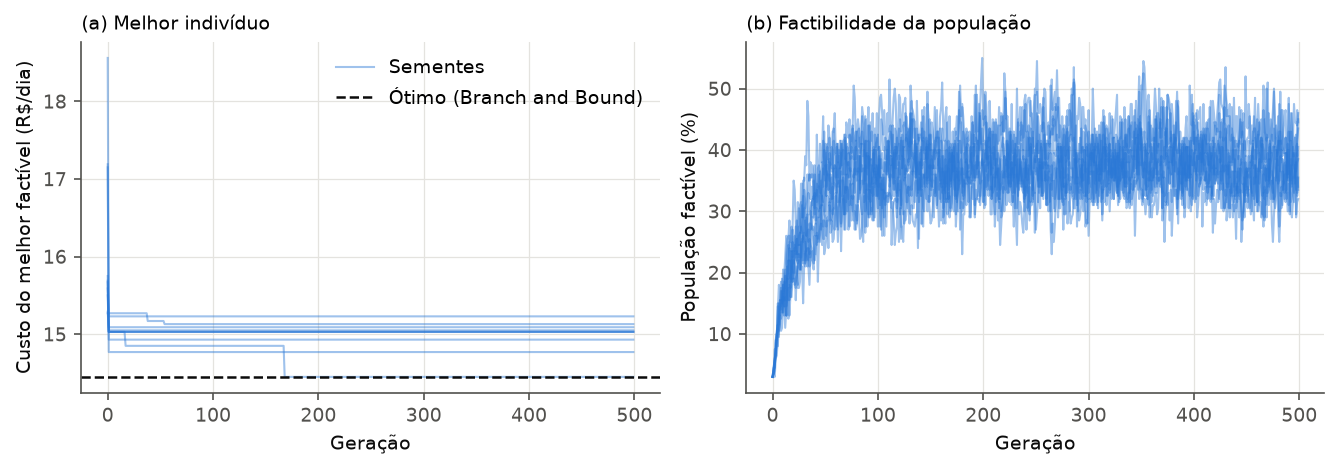
\includegraphics[width=\textwidth]{convergencia_genetico.png}
\caption{Convergência do Algoritmo Genético para o atleta (custo mínimo): (a) custo do
melhor indivíduo factível; (b) fração factível da população.}\label{fig:ga}
\end{figure}

\subsection{Cardápios Gerados}

A Tabela~\ref{tab:cardapio} mostra três cardápios de custo mínimo com porções inteiras,
e a Figura~\ref{fig:composicao}, a origem da energia em cada perfil. Arroz, feijão,
leite e laranja aparecem em quase todos, por serem fontes baratas de energia, proteína,
cálcio e vitamina~C. O fígado entra nos perfis com mais exigência de proteína e ferro,
e o vegano recorre a leguminosas, tofu e bebida de soja. Como todo modelo de custo
mínimo, o resultado tende à monotonia; os limites $M_i$ e a exigência de frutas e
hortaliças reduzem esse efeito.

\begin{table}[ht]
\centering
\caption{Cardápios diários de custo mínimo (porções inteiras).}\label{tab:cardapio}
\footnotesize
\begin{tabular}{p{2.3cm}p{9.7cm}r}
\toprule
Perfil & Cardápio diário (porções) & Custo (R\$) \\
\midrule
Sobrepeso & 1 macarrão cozido; 3 feijão carioca cozido; 2 grão-de-bico cozido; 2 sardinha em conserva; 3 ovo cozido; 2 laranja pera; 1 cenoura crua & 10{,}90 \\[2pt]
Subpeso & 3 arroz branco cozido; 3 arroz integral cozido; 2 macarrão cozido; 3 feijão carioca cozido; 1 sardinha em conserva; 1 leite integral; 1 pasta de amendoim integral; 3 azeite de oliva; 1 laranja pera; 2 couve manteiga refogada; 2 cenoura crua & 12{,}03 \\[2pt]
Atleta & 3 arroz branco cozido; 3 arroz integral cozido; 2 macarrão cozido; 3 feijão carioca cozido; 2 grão-de-bico cozido; 3 ovo cozido; 2 leite desnatado; 3 pasta de amendoim integral; 2 laranja pera; 1 cenoura crua & 14{,}65 \\[2pt]
Vegetariano & 2 arroz branco cozido; 2 arroz integral cozido; 3 feijão carioca cozido; 2 grão-de-bico cozido; 1 ovo cozido; 2 leite integral; 1 azeite de oliva; 2 laranja pera; 2 couve manteiga refogada & 10{,}30 \\[2pt]
Vegano & 3 arroz branco cozido; 1 macarrão cozido; 3 feijão carioca cozido; 2 grão-de-bico cozido; 1 tofu firme; 3 azeite de oliva; 2 laranja pera; 1 cenoura crua & 11{,}30 \\[2pt]
\bottomrule
\end{tabular}

\end{table}

\begin{figure}[ht]
\centering
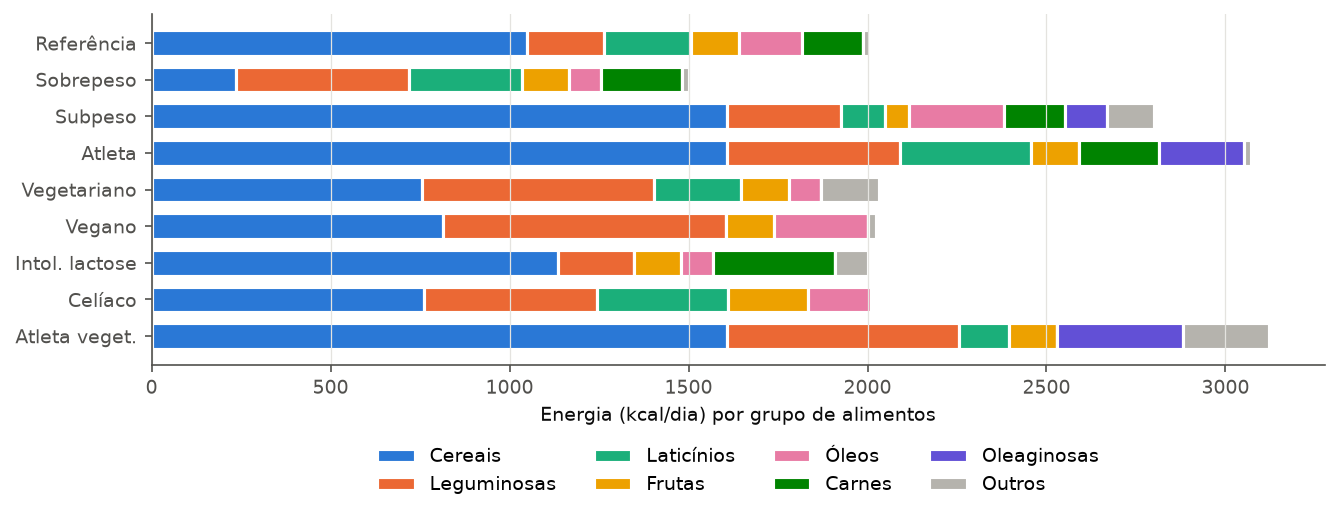
\includegraphics[width=\textwidth]{composicao_cardapios.png}
\caption{Energia por grupo de alimentos nos cardápios de custo mínimo.}\label{fig:composicao}
\end{figure}

\subsection{Custo Computacional}

A Tabela~\ref{tab:tempos} resume os tempos. O Simplex resolve cada instância linear em
milissegundos. O Branch and Bound leva em média %%BB_TEMPO%%~s (no máximo
%%BB_TEMPO_MAX%%~s) e garante o ótimo; o Genético leva %%GA_TEMPO%%~s por execução e
não garante. Parte das execuções dividiu a máquina com outros processos, por isso o
tempo do Genético variou entre cerca de 4 e 11~s; ainda assim, o Branch and Bound foi
mais rápido que o Genético em 25 das 27 instâncias. Neste tamanho de problema (37 variáveis
e até 18 restrições), o Branch and Bound domina o Genético em qualidade e tempo.

\begin{table}[ht]
\centering
\caption{Custo computacional por método.}\label{tab:tempos}
\footnotesize
\begin{tabular}{llrrrr}
\toprule
Método & Modelo & Execuções & Tempo médio & Tempo máximo & Ótimo atingido \\
\midrule
Simplex & linear & 63 & 5{,}7 ms & 19{,}8 ms & 100\% \\
Branch and Bound & inteiro & 27 & 2{,}5 s & 12{,}9 s & 100\% \\
Algoritmo Genético & inteiro & 270 & 7{,}8 s & 11{,}4 s & 14\% \\
\bottomrule
\end{tabular}

\end{table}

\section{Conclusão}\label{sec:conclusao}

Este artigo formulou o problema da dieta para nove perfis com necessidades distintas,
avaliou sete funções objetivo e duas formas de combinar critérios, e resolveu as 90
instâncias por três métodos implementados pelo grupo. O Simplex e o Branch and Bound
coincidiram com o CBC em todas as instâncias; o Genético ficou em média %%GA_GAP%%\%
acima do ótimo. A análise dual mostrou o que encarece cada dieta: proteína para o
atleta, %%DUAL_PROT_PCT%%\% mais cara sem carnes; ferro para o vegetariano; e o teto de
carboidrato no emagrecimento. As fronteiras de Pareto tornam visível a troca entre
custo, proteína e sódio.

O resultado central é que, neste tamanho de problema, os métodos exatos bastam: o
Branch and Bound gera porções que podem ser servidas, com otimalidade garantida, em
poucos segundos. O Genético ganha interesse quando o modelo deixa de ser linear, com
preferências de sabor, regras de combinação entre alimentos ou divisão em refeições.
Os limites nutricionais e os preços são premissas didáticas, e o modelo não substitui
um nutricionista. Trabalhos futuros podem ampliar a base de alimentos e nutrientes
(vitamina B12, zinco, ômega-3) e incluir essas preferências.

\bibliographystyle{sbc}
\bibliography{referencias}

\end{document}
